\chapter{Measurements}\label{chap:measurements}

In order to test the detector and crystal response, multiple electronic setups were used to obtain spectra from calibrated sources. This chapter summarizes the most important measurements achieved while testing the CosmicWatch, showcasing some features that are yet to be understood.

\section{Rohde\&Schwarz RTO6 oscilloscope}

The Rohde\&Schwarz RTO6 oscilloscope was the main troubleshooting tool used to test the detector as a whole. The histogram functionality on the oscilloscope allowed us to also measure spectra from calibrated sources, Figure \ref{fig:RS_spectra} shows the obtained spectra. The $x$ axis measures SiPM pulse areas since the oscilloscope creates histograms based on the area under each SiPM pulse (\textcolor{blue}{blue} signal in Fig. \ref{fig:signal_processing}).

It is important to note here the shape of the background (Fig. \ref{sfig:RS_bkgd}), remembering Figure \ref{fig:LYSO_background}, a sudden increase in intensity should occur at around 290 and 597 \unit{\kilo\eV}, therefore the 511 \unit{\kilo\eV} peak of $^{22}$Na should lie in between these values, while 662 \unit{\kilo\eV} from $^{137}$Cs would lie above the second increase in background counts. These approximations can help us get a notion of what we are seeing in the various spectra illustrated in Fig. \ref{fig:RS_spectra}.

The highest peak in $^{137}$Cs is presumed to be caused by x-ray emissions from lower shell electrons filling the space left by internal conversion electrons, this peak is also featured in Figure \ref{fig:Cs137_description}. One important feature in the cesium spectrum is the relatively high intensities passed the photopeak (at 47.57(1) nVs according to the gaussian fit), this is not due to LYSO background since these counts greatly exceed the expected background.

\begin{figure}[H]
  \begin{subfigure}[t]{0.48\textwidth}
    \centering
    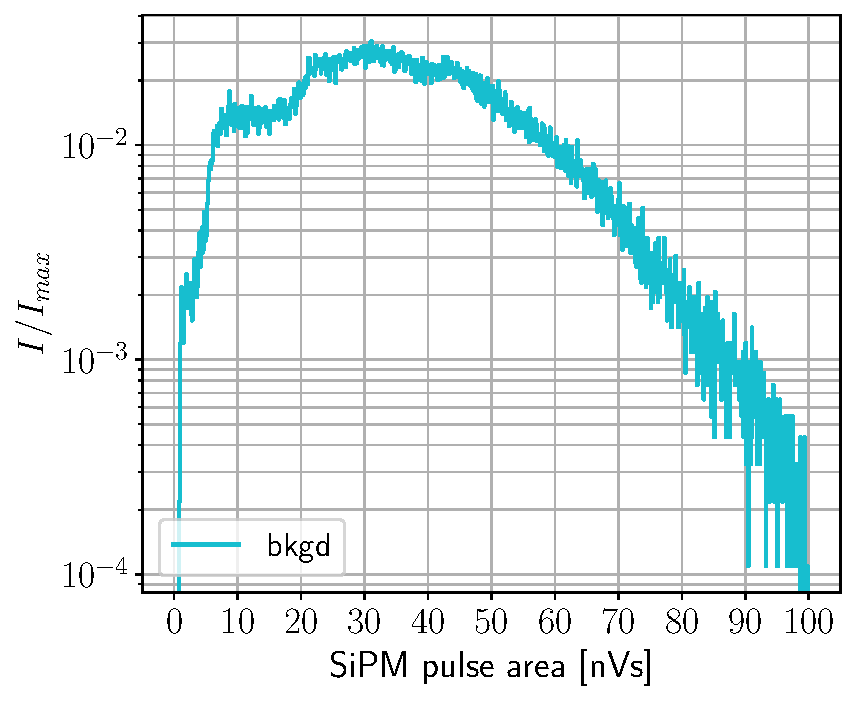
\includegraphics[width=\textwidth]{measurements/RS/teflon-bkgd.pdf}
    \caption{\label{sfig:RS_bkgd}LYSO background.}
  \end{subfigure}
  \hfill
  \begin{subfigure}[t]{0.48\textwidth}
    \centering
    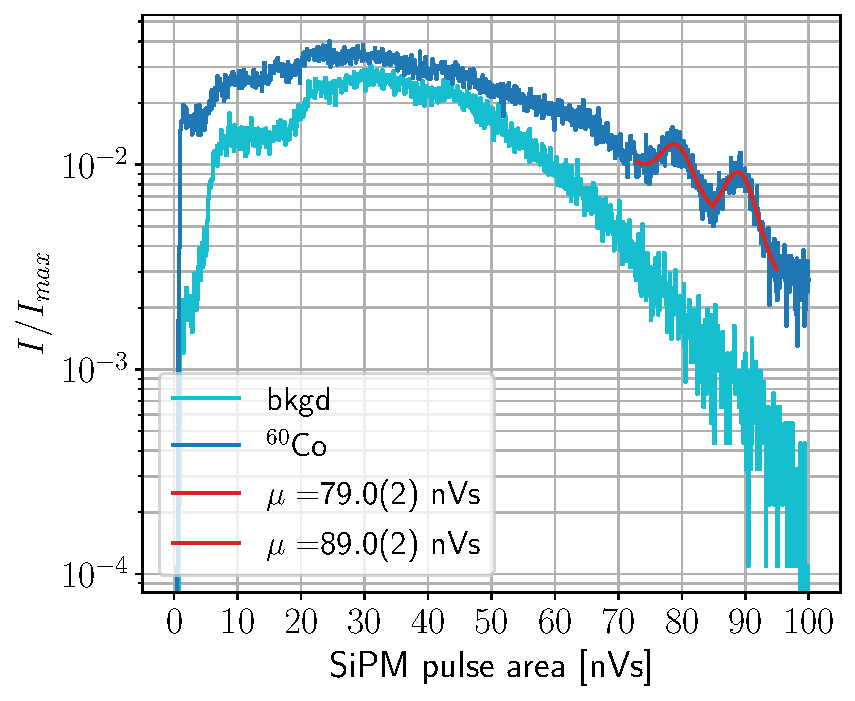
\includegraphics[width=\textwidth]{measurements/RS/teflon-side-Co60.pdf}
    \caption{\label{sfig:RS_60Co}$^{60}$Co.}
  \end{subfigure}
  \medskip
  \begin{subfigure}[t]{0.48\textwidth}
    \centering
    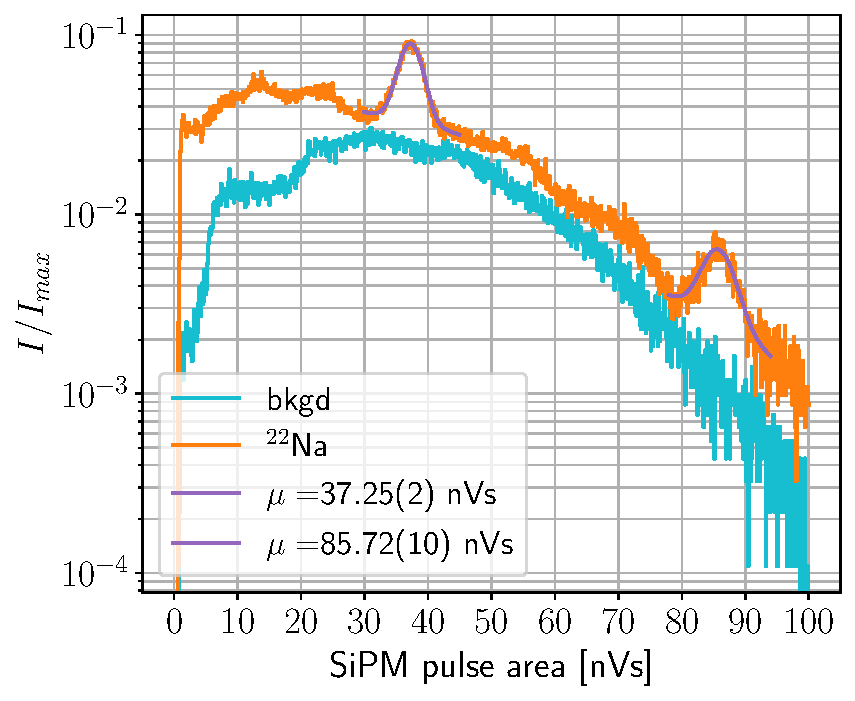
\includegraphics[width=\textwidth]{measurements/RS/teflon-side-Na22.pdf}
    \caption{\label{sfig:RS_22Na}$^{22}$Na.}
  \end{subfigure}
  \hfill
  \begin{subfigure}[t]{0.48\textwidth}
    \centering
    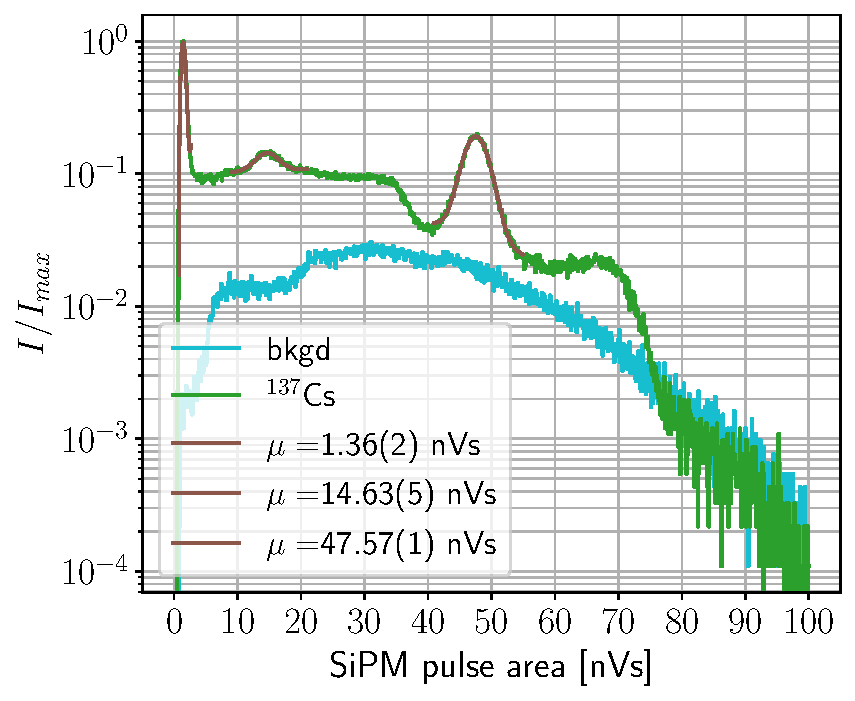
\includegraphics[width=\textwidth]{measurements/RS/teflon-side-Cs137.pdf}
    \caption{\label{sfig:RS_137Cs}$^{137}$Cs.}
  \end{subfigure}
  \caption{\label{fig:RS_spectra}Spectra measured with the histogram functionality of a Rohde\&Schwarz RTO6 oscilloscope. Each graph features the centroid of the Gaussian fitted to each peak.}
\end{figure}

Fitting gaussian functions to the main peaks one can get the relation between energy and pulse area (Fig. \ref{sfig:RS_LYSO_calibration_low_peaks}) based on the decay schemes shown in Figure \ref{fig:decay_schemes}. Considering the x-ray and backscattering peaks of $^{137}$Cs, however, seems to cause an overestimation of the energies, as can be seen in Figure \ref{sfig:RS_LYSO_calibrated_spectrum_low_peaks}, where the pair-production peak of sodium, for example, lies at 535.95 keV instead of 511 keV. The calibration shown in Figure \ref{sfig:RS_LYSO_calibration} does not take into account the troublesome peaks of Cesium, better estimating high energy peaks, this however results in negative-energy predictions at the lower energy range in the spectrum.

\begin{figure}[H]
  \begin{subfigure}[t]{\textwidth}
    \centering
    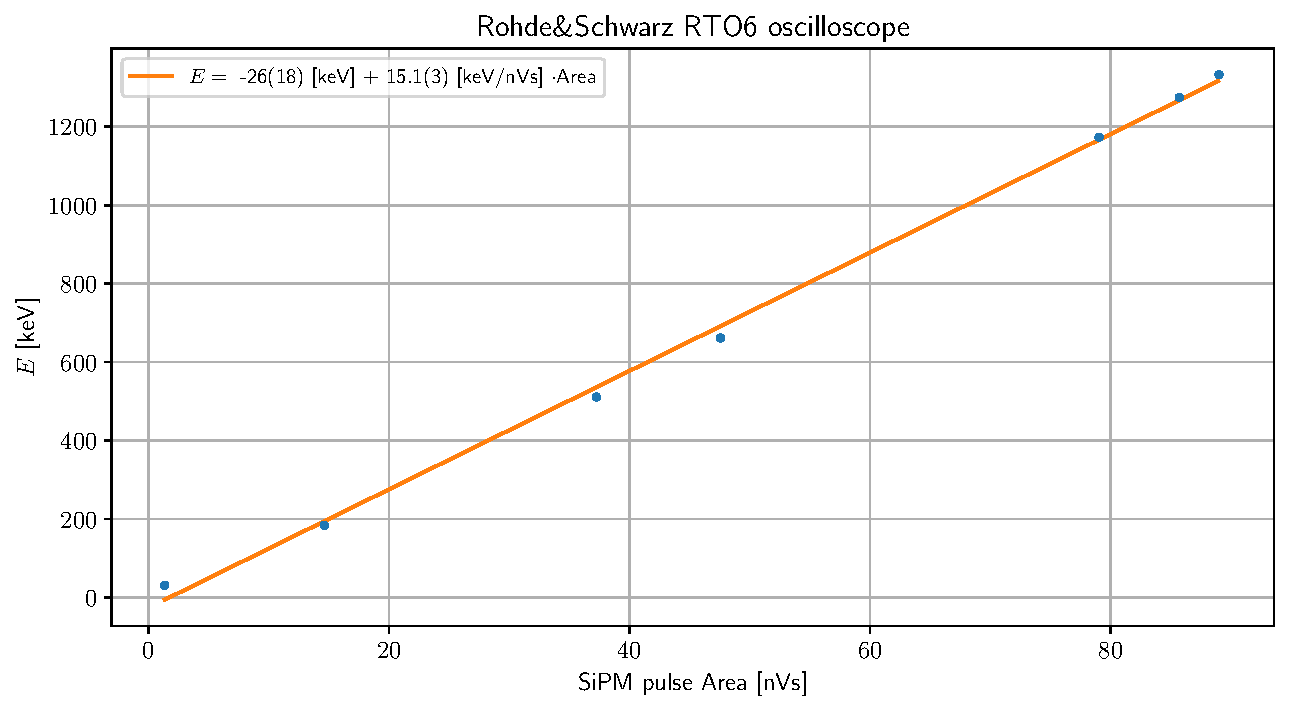
\includegraphics[width=.98\textwidth]{measurements/RS/LYSO_calibration_low_peaks.pdf}
    \caption{\label{sfig:RS_LYSO_calibration_low_peaks}LYSO calibration from Rohde\&Schwarz oscilloscope. Obtained by fitting gaussian functions to the main peaks shown in Fig \ref{sfig:RS_60Co}, \subref{sfig:RS_22Na}, and \subref{sfig:RS_137Cs}.}
  \end{subfigure}
  \medskip
  \begin{subfigure}[t]{\textwidth}
    \centering
    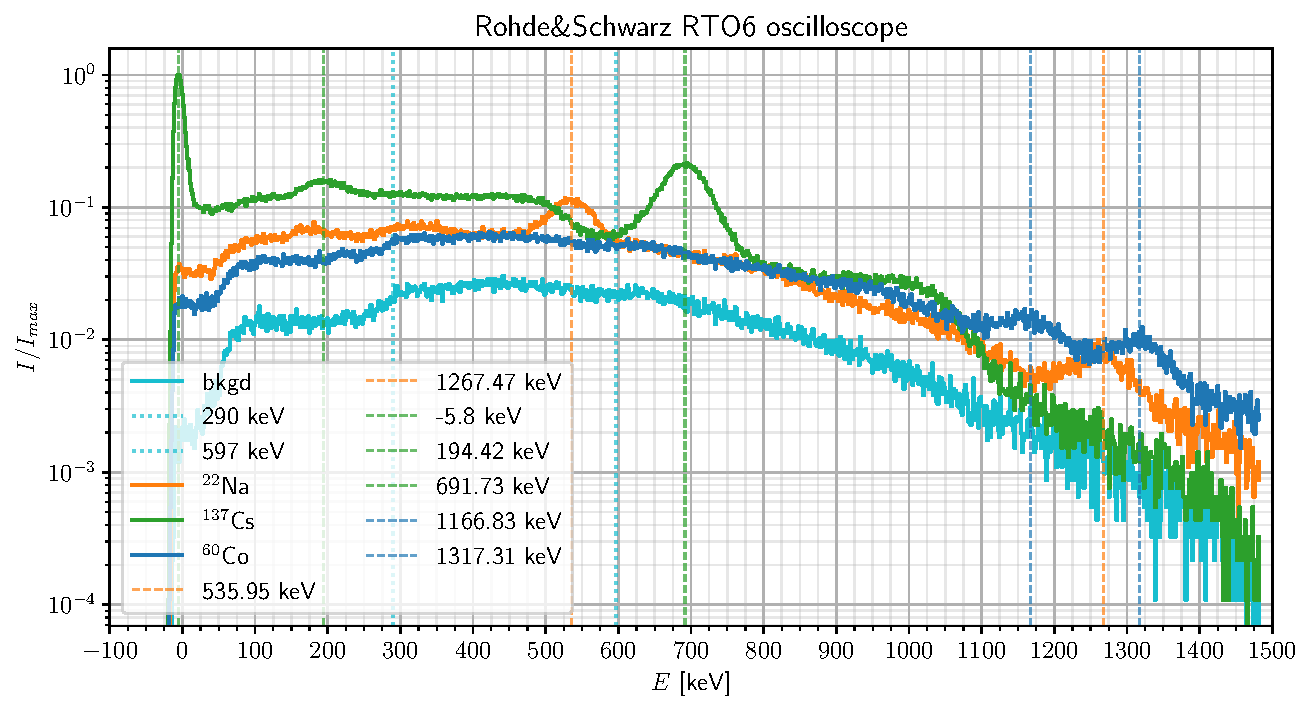
\includegraphics[width=.98\textwidth]{measurements/RS/Calibrated_spectrum_low_peaks.pdf}
    \caption{\label{sfig:RS_LYSO_calibrated_spectrum_low_peaks}Calibrated spectrum obtained from the channel-energy conversion shown in \subref{sfig:RS_LYSO_calibration_low_peaks}.}
  \end{subfigure}
  \caption{\label{fig:RS_low_peaks_calibration}Calibrated spectrum taking into account the x-ray and backscattering peaks of $^{137}$Cs.}
\end{figure}

\begin{figure}[H]
  \begin{subfigure}[t]{\textwidth}
    \centering
    \includegraphics[width=.98\textwidth]{measurements/RS/LYSO_calibration.pdf}
    \caption{\label{sfig:RS_LYSO_calibration}LYSO calibration from Rohde\&Schwarz oscilloscope. Excluding x-ray and backscattering peaks from \subref{sfig:RS_137Cs}.}
  \end{subfigure}
  \medskip
  \begin{subfigure}[t]{\textwidth}
    \centering
    \includegraphics[width=.98\textwidth]{measurements/RS/Calibrated_spectrum.pdf}
    \caption{\label{sfig:RS_LYSO_calibrated_spectrum}Calibrated spectrum obtained from the channel-energy conversion shown in \subref{sfig:RS_LYSO_calibration}.}
  \end{subfigure}
  \caption{\label{fig:RS_calibration}Calibrated spectrum, ignoring the x-ray and backscattering peaks of $^{137}$Cs.}
\end{figure}

In general, the $\chi^2$ results for the multiple fits performed were much better while ignoring the low energies of Cesium, leading us to conclude that this might be optimal, obtaining the final FWHM vs Energy calibration shown in Fig. \ref{fig:RS_FWHM}. This results in an energy resolution of 13.5\% at 511 keV.

\begin{figure}[H]
  \centering
  \includegraphics[width=.98\textwidth]{measurements/RS/FWHM.pdf}
  \caption{\label{fig:RS_FWHM}FWHM as a function of energy from spectra obtained with a Rohde\&Schwarz RTO6 oscilloscope.}
\end{figure}

\section{CosmicWatch electronics}

\section{NIM modules}

In the same way the CosmicWatch was studied with the Rohde\&Schwarz oscilloscope, NIM modules were used to get a LYSO calibration when coupled to the SiPM, this section shows some of the results obtained.

\subsection{Odd features}

While testing the detector response some odd features were found in the measured spectra, they are yet to be understood and present an interesting study case, Figure \ref{fig:NIM_odd_features} showcases some of the spectra obtained that illustrate these anomalies. 

$^{54}$Mn, is a monoenergetic source, meaning that it only produces one gamma ray, in this case at 835 \unit{\kilo\eV}, which lies slightly above 662 \unit{\kilo\eV} ($^{137}$Cs), therefore, the peak in channel 259 in Fig. \ref{sfig:NIM_odd_54Mn} should correspond to the gamma emission from Manganese. However, there is again a very high number of events above the photopeak, which is not expected, since 835 \unit{\kilo\eV} is the maximum energy one should see in this spectrum. Aside from this, it is also clear that the shape of this peak does not fully adjust to a gaussian distribution, showing that there is an underlying structure that has not been explained. These odd features can also be seen in $^{137}$Cs.

\begin{figure}[H]
  \centering
  \begin{subfigure}[t]{0.53\textwidth}
    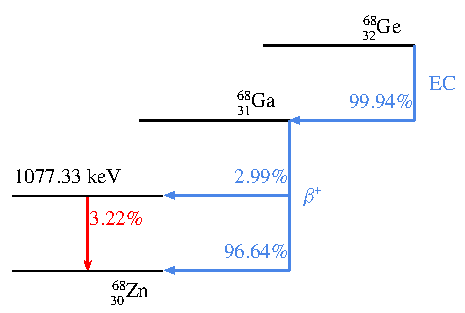
\includegraphics[width=\textwidth]{measurements/68Ge-decay.pdf}
    \caption{\label{sfig:68Ge_decay_scheme}}
  \end{subfigure}
  \begin{subfigure}[t]{0.425\textwidth}
    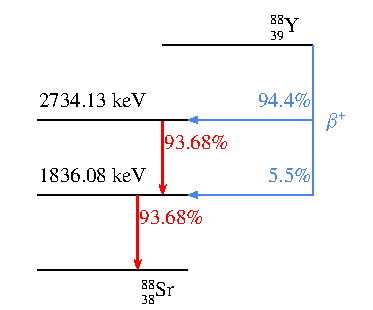
\includegraphics[width=\textwidth]{measurements/88Y-decay.pdf}
    \caption{\label{sfig:88Y_decay_scheme}}
  \end{subfigure}
  \caption{\label{fig:some_decay_schemes}Decay schemes for $^{68}$Ge and $^{88}$Y}
\end{figure}

In principle, $^{68}$Ge should have a spectrum very similar to $^{22}$Na, in this case, however, the decay chain most often ends in a stable state of $^{68}$Zn as illustrated in Fig. \ref{sfig:68Ge_decay_scheme}, this means that the only appreciable peak should lie at 511 \unit{\kilo\eV}, due to pair production from the 1077.33 \unit{\kilo\eV} gamma emission and the subsequent positron annihilation. This agrees with Fig. \ref{sfig:NIM_odd_68Ge}, notably, however, there are very few counts at energies above 511 \unit{\kilo\eV}, which is not the case for the other sources, they present high counts above their respective photopeak. This may be due to the low activity of the source. 

\begin{figure}[H]
  \begin{subfigure}[t]{0.47\textwidth}
    \centering
    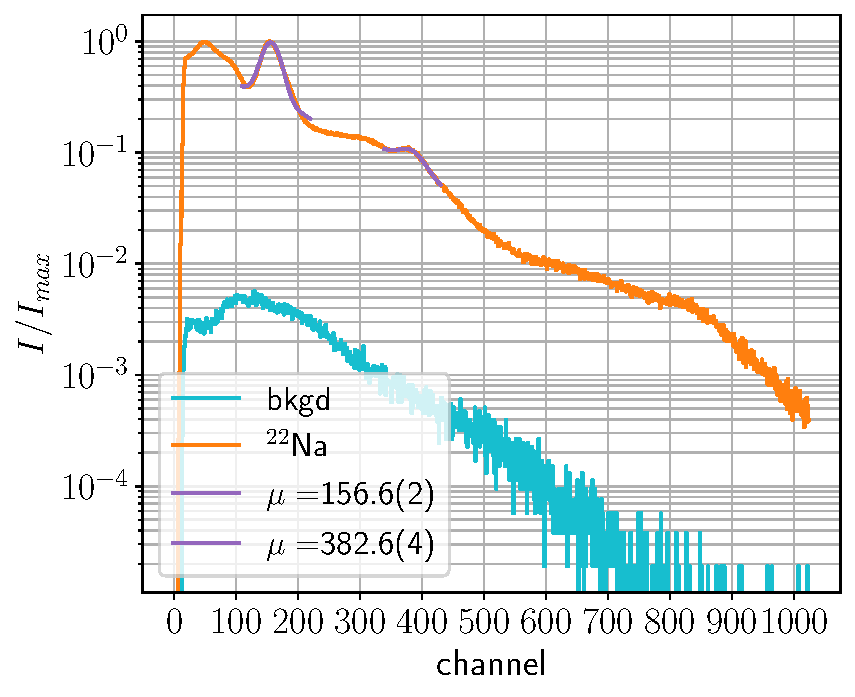
\includegraphics[width=\textwidth]{measurements/NIM/odd_features/22Na.pdf}
    \caption{\label{sfig:NIM_odd_22Na}$^{22}$Na, $A=1697.320$ kBq.}
  \end{subfigure}
  \hfill
  \begin{subfigure}[t]{0.47\textwidth}
    \centering
    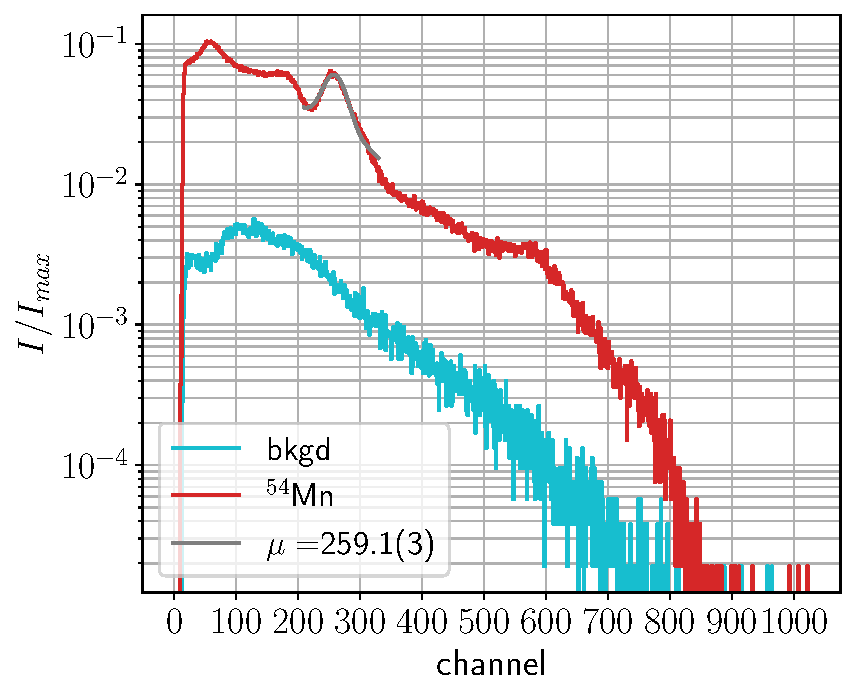
\includegraphics[width=\textwidth]{measurements/NIM/odd_features/54Mn.pdf}
    \caption{\label{sfig:NIM_odd_54Mn}$^{54}$Mn, $A=623.108$ kBq.}
  \end{subfigure}
  \medskip
  \begin{subfigure}[t]{0.47\textwidth}
    \centering
    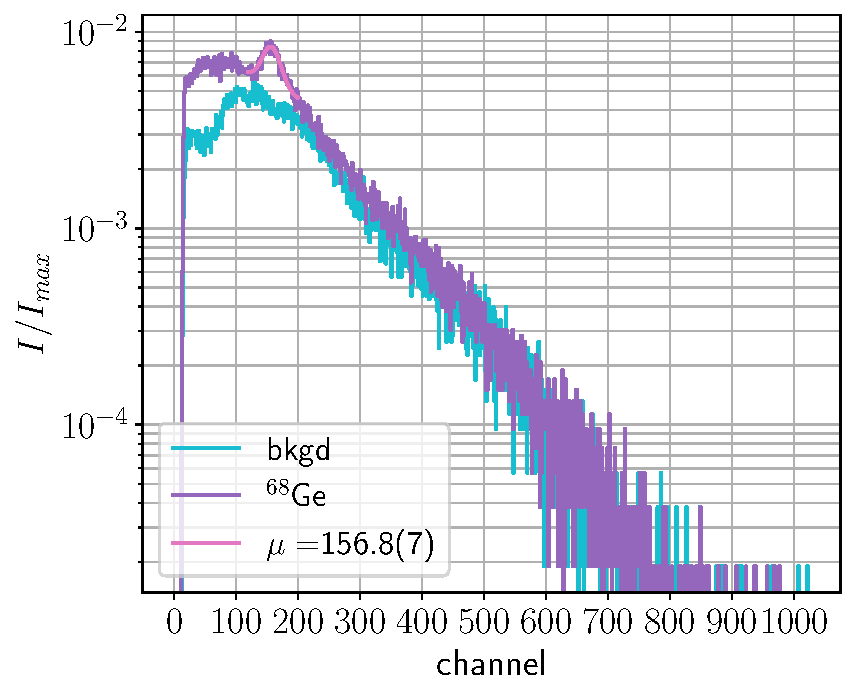
\includegraphics[width=\textwidth]{measurements/NIM/odd_features/68Ge.pdf}
    \caption{\label{sfig:NIM_odd_68Ge}$^{68}$Ge, $A=$? kBq.}
  \end{subfigure}
  \hfill
  \begin{subfigure}[t]{0.47\textwidth}
    \centering
    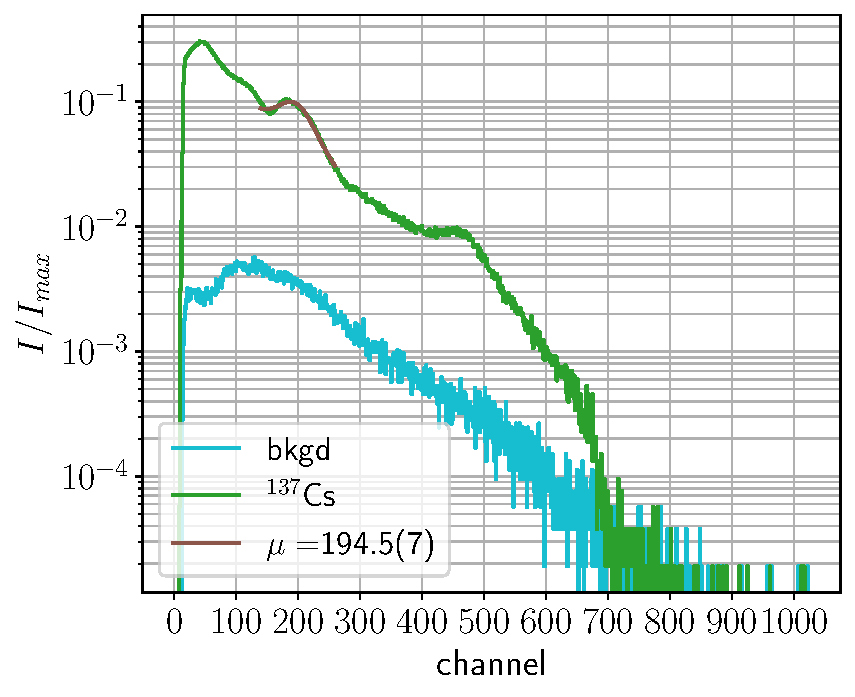
\includegraphics[width=\textwidth]{measurements/NIM/odd_features/137Cs_HA.pdf}
    \caption{\label{sfig:NIM_odd_137Cs}$^{137}$Cs, $A=30790.372$ kBq.}
  \end{subfigure}
  \caption{\label{fig:NIM_odd_features}Spectra measured with a Timing Filter Amplifier and Analog to Digital Converter NIM modules. Each graph features the isotope used, its activity at the time of measurement, and the centroid of the Gaussian fitted to each peak. The $x$ axis gives channels since the ADC creates a histogram based on pulse area. Some odd features can be seen in these spectra, like the large number of counts above the Cesium and Manganese photopeaks.}
\end{figure}

\begin{figure}[H]
  \centering
  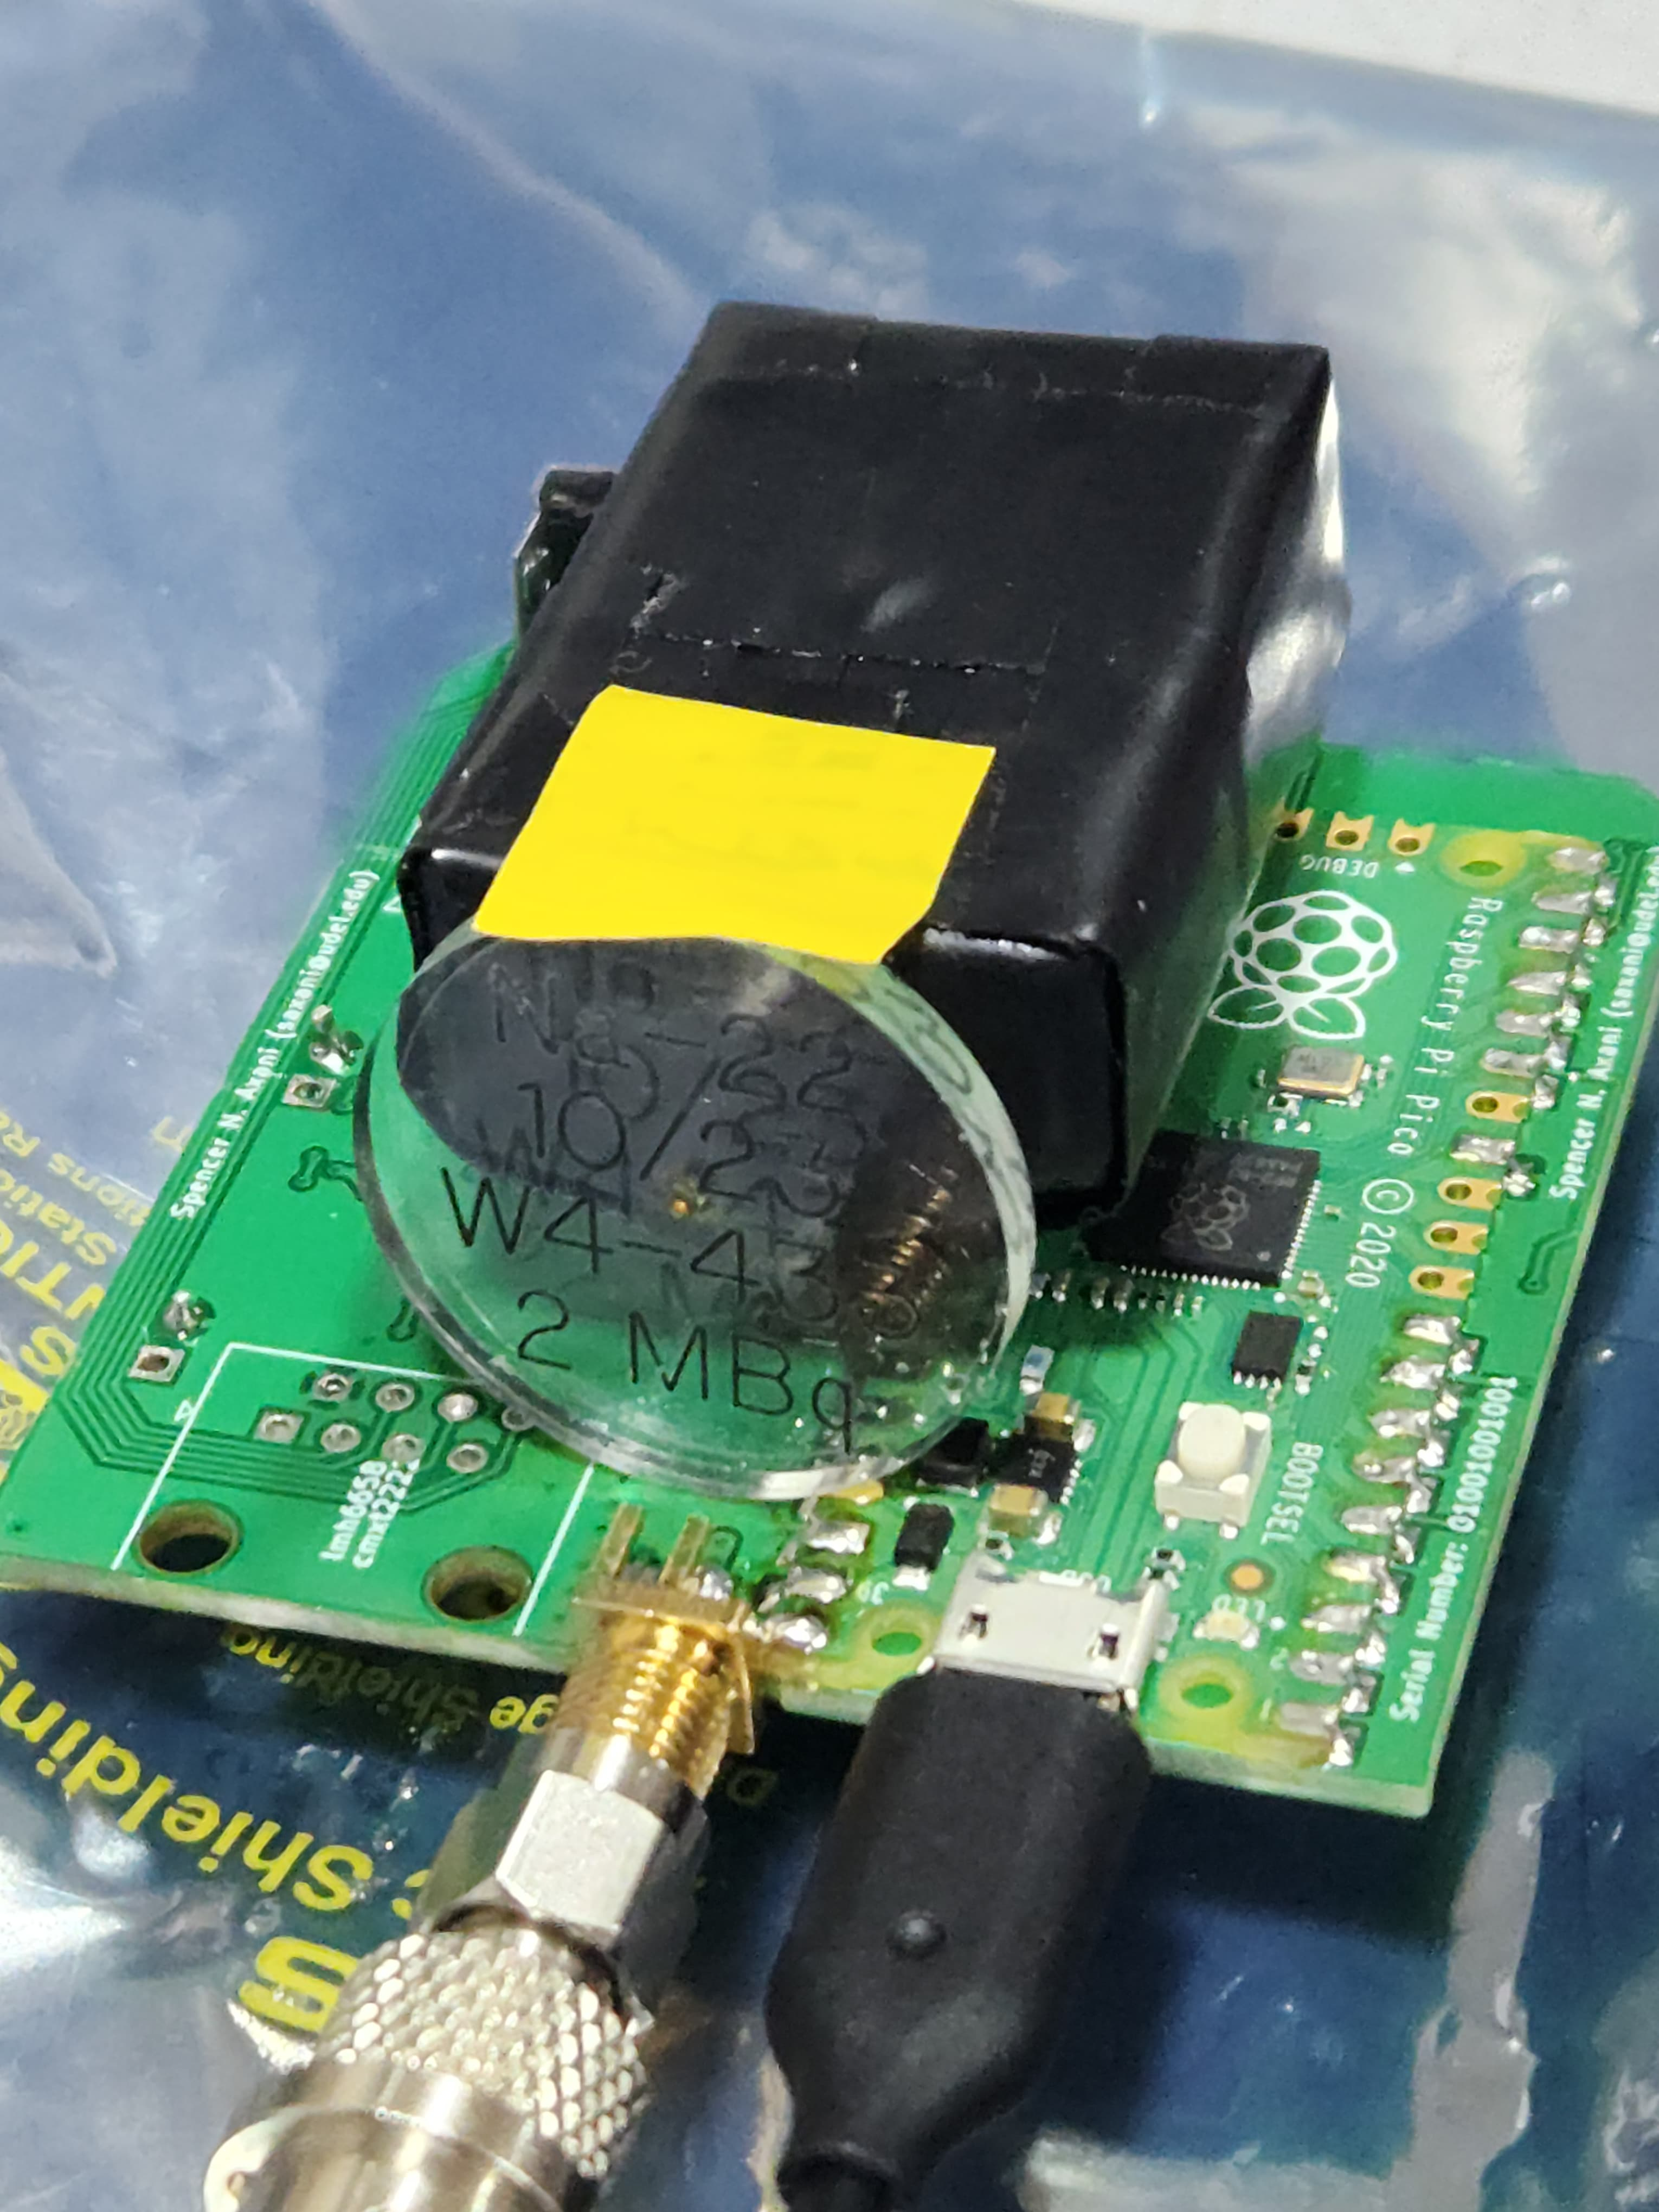
\includegraphics[width=.3\textwidth]{measurements/Source_position.jpg}
  \caption{\label{fig:source_position}Source positioning relative to the detector.}
\end{figure}

Figure \ref{fig:source_position} shows how the radioactive source is positioned relative to the detector, it is done this way for two reasons: first, it ensures the gamma rays will have a longer travel path inside the crystal, and second, because moving the source away from the crystal greatly decreased the resolution. The Cesium spectrum shown in Fig. \ref{sfig:NIM_odd_137Cs} was taken while placing the source 10 cm away from the detector, trying to reduce the count rate due to the large activity of the source, nonetheless, this resulted on an oddly shaped photopeak, as showcased in the comparatively large FWHM at 662 keV shown in Fig \ref{fig:NIM_odd_FWHM}.  

\begin{figure}[H]
  \centering
  \includegraphics[width=.98\textwidth]{measurements/NIM/odd_features/FWHM.pdf}
  \caption{\label{fig:NIM_odd_FWHM}FWHM obtained from gaussian fits to the photo- and positron-annihilation peaks shown in \ref{fig:NIM_odd_features}.}
\end{figure}

\subsection{Calibration}

Following the goal of this work, multiple spectra were measured trying to find the NIM-modules setup that would optimize energy resolution. As expressed in \cite[sec.~4.4.3]{gilmore2008practical}: ``theory suggests that the lowest noise contribution is found when the integration and differentiation times are made equal. On all modern amplifiers, the shaping time constants are made equal and are controlled by a single selector knob.'' In our case, however, the integration and differentiation times were controlled independently, since we used a Canberra Model 2111 Timing Filter Amplifier \cite{CanberraTFA}. So far, the best results were found while using the OUT setup for both time constants, corresponding to 4 ns of integration time and 160 $\mu$s of differentiation time. 

Even though the FWHM does not vary significantly for different time-constant setups, the OUT configuration produced the most accurate calibrations achieved, obtaining an energy resolution of 25.2\% at 511 keV. Further work needs to be done to better understand the origin of the odd features presented above, this may greatly influence the energy resolution since, as can be seen in the Manganese spectrum, not all the peaks present a truly gaussian form.

\begin{figure}[H]
  \centering
  \includegraphics[width=.98\textwidth]{measurements/NIM/2024-05-24/outD/FWHM.pdf}
  \caption{\label{fig:NIM_FWHM}FWHM obtained from gaussian fits to the photo- and positron-annihilation peaks shown in \ref{fig:NIM_spectra}.}
\end{figure}

It is worth noting the great similarities between Figures \ref{sfig:NIM_54Mn}-\subref{sfig:NIM_88Y} and the features explained in subsection \ref{sec:gammas_in_the_detector}, each showcasing a clear photopeak, Compton edge, and backscattering peak.

\begin{figure}[H]
  \begin{subfigure}[t]{0.47\textwidth}
    \centering
    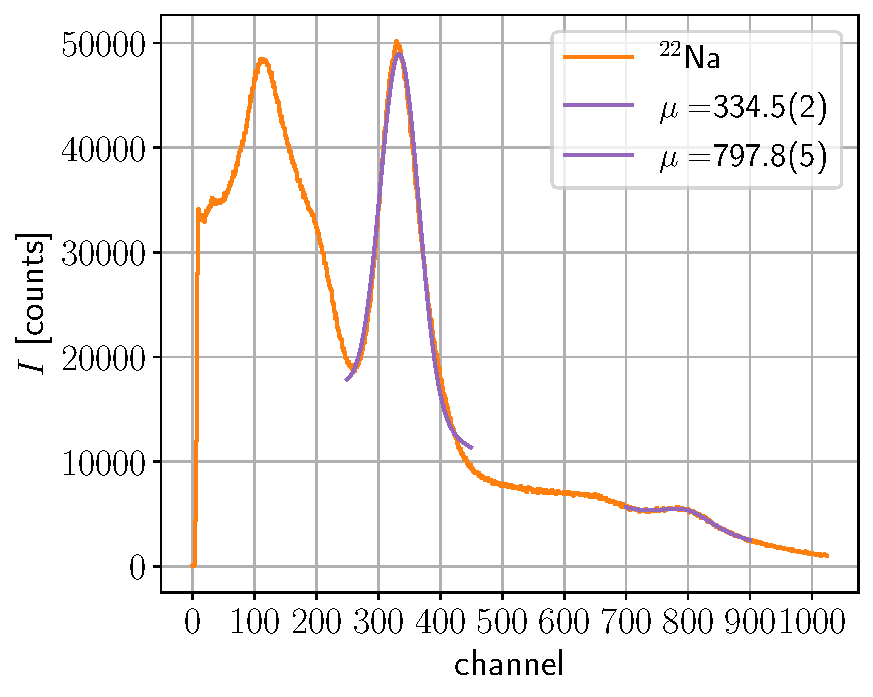
\includegraphics[width=\textwidth]{measurements/NIM/2024-05-24/outD/outD_22Na.pdf}
    \caption{\label{sfig:NIM_22Na}$^{22}$Na, $A=1697.320$ kBq.}
  \end{subfigure}
  \hfill
  \begin{subfigure}[t]{0.47\textwidth}
    \centering
    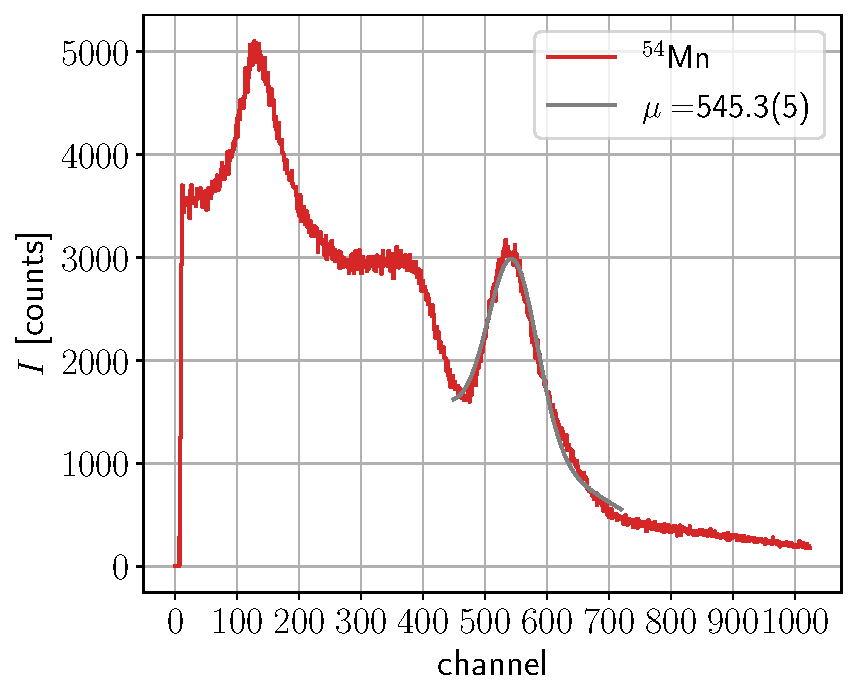
\includegraphics[width=\textwidth]{measurements/NIM/2024-05-24/outD/outD_54Mn.pdf}
    \caption{\label{sfig:NIM_54Mn}$^{54}$Mn, $A=623.108$ kBq.}
  \end{subfigure}
  \medskip
  \begin{subfigure}[t]{0.47\textwidth}
    \centering
    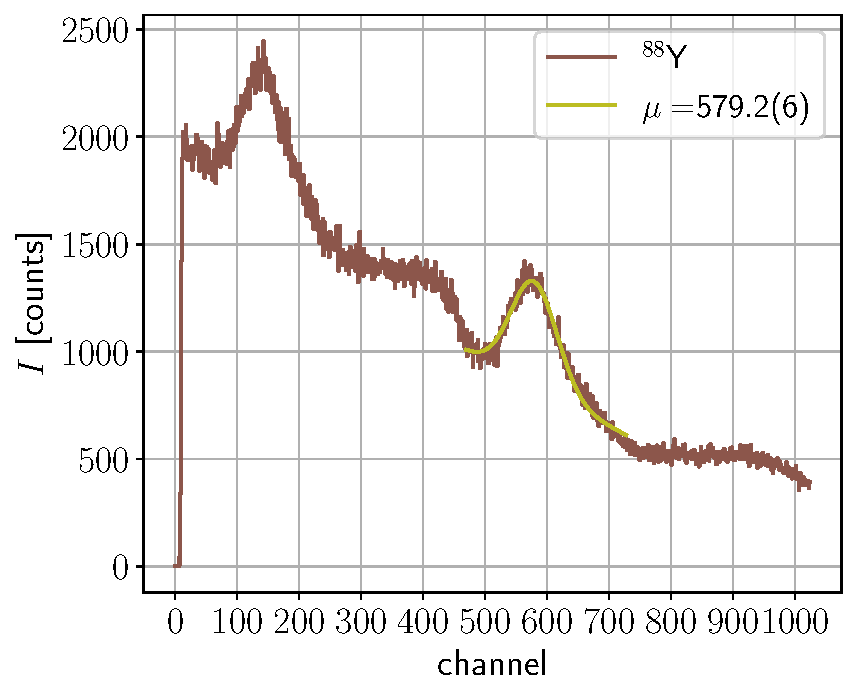
\includegraphics[width=\textwidth]{measurements/NIM/2024-05-24/outD/outD_88Y.pdf}
    \caption{\label{sfig:NIM_88Y}$^{88}$Y, $A=251.980$ kBq.}
  \end{subfigure}
  \hfill
  \begin{subfigure}[t]{0.47\textwidth}
    \centering
    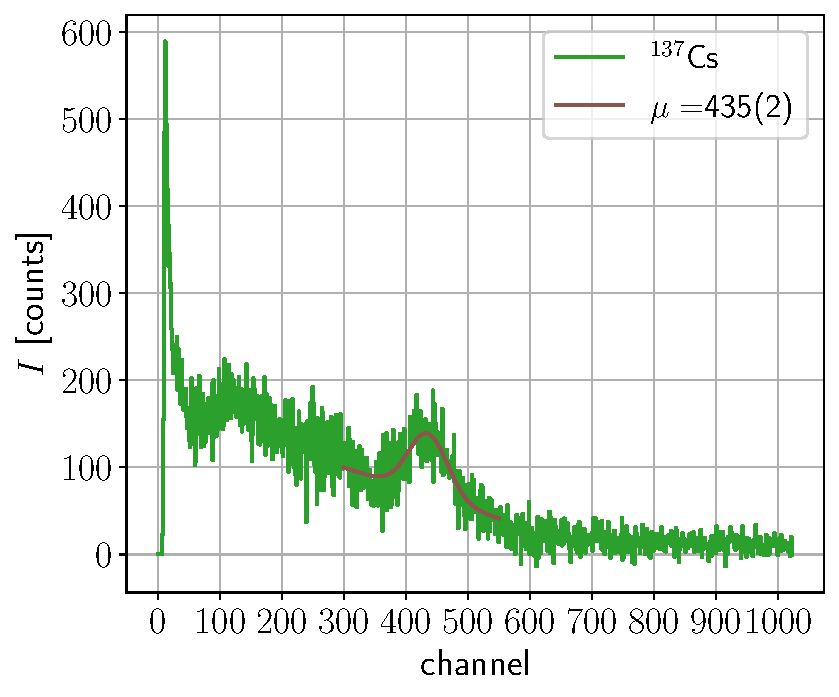
\includegraphics[width=\textwidth]{measurements/NIM/2024-05-24/outD/outD_137Cs.pdf}
    \caption{\label{sfig:NIM_137Cs}$^{137}$Cs, $A=23.139$ kBq.}
  \end{subfigure}
  \caption{\label{fig:NIM_spectra}Spectra measured with a Timing Filter Amplifier and Analog to Digital Converter NIM modules. The $x$ axis measures channels since the ADC creates a histogram based on pulse area. Each graph features the centroid of the Gaussian fitted to each peak.}
\end{figure}

\begin{figure}[H]
  \begin{subfigure}[t]{\textwidth}
    \centering
    \includegraphics[width=.98\textwidth]{measurements/NIM/2024-05-24/outD/LYSO_calibration.pdf}
    \caption{\label{sfig:NIM_LYSO_calibration}LYSO calibration from NIM modules. Obtained by fitting gaussian functions to the main peaks shown in Fig \ref{sfig:NIM_54Mn} to \subref{sfig:NIM_137Cs}.}
  \end{subfigure}
  \medskip
  \begin{subfigure}[t]{\textwidth}
    \centering
    \includegraphics[width=.98\textwidth]{measurements/NIM/2024-05-24/outD/Calibrated_spectrum.pdf}
    \caption{\label{sfig:NIM_LYSO_calibrated_spectrum}Calibrated spectrum obtained from the channel-energy conversion shown in \subref{sfig:NIM_LYSO_calibration}.}
  \end{subfigure}
  \caption{\label{fig:NIM_calibration}Calibrated spectrum.}
\end{figure}

Notably, this new calibration does not result in the prediction of negative energies, like in the case of the RTO6 oscilloscope, despite the various flaws in these spectra.